% standalone document border convention: {left bottom right top}
\documentclass[varwidth=425pt,border={0pt, 1pt, 0pt, 0.5pt}]{standalone}
\usepackage[force]{feynmp-auto}		    
\usepackage{amsmath}
\usepackage{graphicx}

\begin{document}
\begin{equation*}
	\Gamma^{(3)}_{123} \hspace*{0.5ex}=\hspace*{0.5ex}
	\delta_{123}
	\left(\hspace*{-0.5ex}
	\scalebox{0.75}{$
			\begin{gathered}
				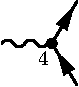
\includegraphics{gamma3/gamma3_0.pdf}
			\end{gathered}
		$}
	\hspace*{0.25ex}\right)
	\hspace*{0.5ex}+\hspace*{0.5ex}
	\delta_{23}
	\left(\hspace*{-0.5ex}
	\scalebox{0.75}{$
			\begin{gathered}
				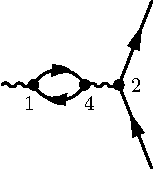
\includegraphics{gamma3/gamma3_1a.pdf}
			\end{gathered}
		$}
	\hspace*{0.25ex}\right)
	\hspace*{0.5ex}+\hspace*{0.5ex}
	\scalebox{0.75}{$
			\begin{gathered}
				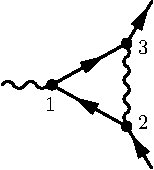
\includegraphics{gamma3/gamma3_1b.pdf}
			\end{gathered}
		$}
	\hspace*{0.5ex}+\hspace*{0.5ex} \cdots
\end{equation*}
\end{document}
